\documentclass[12pt,a4paper]{article}
\usepackage[utf8]{inputenc}
\usepackage[margin=1in]{geometry}
\usepackage{amsmath,amsfonts,amssymb}
\usepackage{graphicx}
\usepackage{tikz}
\usepackage{pgfplots}
\usepackage{float}
\usepackage{cite}
\usepackage{url}
\usepackage{setspace}
\usepackage{fancyhdr}
\usepackage{titlesec}
\usepackage{booktabs}
\usepackage{xcolor}

% Configure page style
\pagestyle{fancy}
\fancyhf{}
\rhead{Digital Assignment}
\lhead{22MIA1103}
\cfoot{\thepage}

% Configure section formatting
\titleformat{\section}{\large\bfseries}{\thesection}{1em}{}
\titleformat{\subsection}{\normalsize\bfseries}{\thesubsection}{1em}{}

\onehalfspacing

\begin{document}

% Title Page
\begin{titlepage}
\centering
\vspace*{2cm}

{\LARGE\bfseries SDG 13 (Climate Action)}\\[1cm]
{\large CSE4077 - Recommender Systems Journal Report}\\[0.5cm]
{\normalsize Submitted to: Dr. Manjula V}\\[1.5cm]

\vspace{2cm}
\begin{tabular}{ll}
\textbf{Student Name:} & Raazi Faisal Mohiddin \\
\textbf{Registration Number:} & 22MIA1103 \\
\textbf{Course:} & CSE4077 Recommender Systems \\
\textbf{SDGs Covered:} & SDG 13 (Climate Action) \\
\textbf{Submission Date:} & \today \\
\end{tabular}

\vspace*{7cm}

% VIT Logo
\includegraphics[width=0.6\textwidth]{vit_logo_colored-1536x438.png}\\[0.75cm]

{\large School of Computer Science and Engineering}\\
{\large Vellore Institute of Technology, Chennai}\\
\end{titlepage}

\newpage
\tableofcontents
\newpage

\section{Executive Summary}

Using AI to solve major global challenges sounds great in theory, but reality proves much more complex than researchers often acknowledge. This analysis examines how recommendation systems are being adapted to address Sustainable Development Goals. These are the same algorithms typically used for content suggestions. The results reveal both promising innovations and significant limitations.

Two distinct approaches were examined. The first attempts to address educational inequality through intelligent learning resource recommendations for underserved communities. The system achieves 78\% user satisfaction rates through sophisticated collaborative filtering. Deeper analysis reveals fundamental challenges. Students from different cultural backgrounds, such as those in rural Kenya, encounter systems designed with different cultural assumptions. Researchers recognize this "cultural adaptation challenge," but their proposed solutions appear insufficient.

The second study focuses on climate action through predictive modeling of sustainable behavior adoption. Technical achievements are notable. The system achieves 85\% accuracy in behavior prediction using deep learning methods. A critical disconnect emerges. Recommending public transit proves meaningless in areas lacking adequate transportation infrastructure. The gap between algorithmic recommendations and practical implementation possibilities creates significant limitations.

Comparative analysis identifies three recurring problems. These systems demonstrate effectiveness within specific contexts but lack broader applicability. They assume reliable internet connectivity and modern devices. These assumptions fail for many communities requiring SDG interventions. Most concerning, success metrics focus on system engagement rather than actual progress toward sustainability objectives.

The proposed solution involves fundamentally restructuring the approach. Rather than developing sophisticated systems for ideal conditions, development should begin with real-world constraints. Community-centered algorithms need to work offline. They also need genuine impact measurement that tracks real problem-solving progress. This approach could potentially increase engagement by 40\% while functioning effectively in resource-constrained environments.

\section{Introduction to SDG Context}

\subsection{The Role of Recommendation Systems in Sustainable Development}

The technology behind product recommendations now targets world hunger and climate change. These algorithms that suggest sneakers or movies are being repurposed for social good. This represents an intriguing development in applied technology.

The underlying concept appears logical. Recommendation systems excel at understanding individual preferences and needs. Extending this capability to connect rural students with educational resources or guide sustainable behavior adoption seems promising theoretically.

Significant complexity emerges upon closer examination. Commercial success metrics prove straightforward. Purchase completion indicates effectiveness. Addressing global poverty or climate change requires entirely different success definitions and measurement approaches.

Commercial recommendation systems optimize for clear metrics: clicks, purchases, engagement time. SDG-aligned systems must balance effectiveness, community fairness, cultural sensitivity, and lasting positive impact. These requirements create substantially more complex evaluation frameworks than simple transaction completion.

This shift represents more than technical adaptation. It demands a fundamental philosophical change. Algorithms must transition from encouraging individual consumption to facilitating community-wide behavioral change for collective benefit. Such transformation challenges core assumptions about technology's role and purpose.

% Mermaid-style diagram showing SDG-Recommendation System Integration
\begin{figure}[H]
\centering
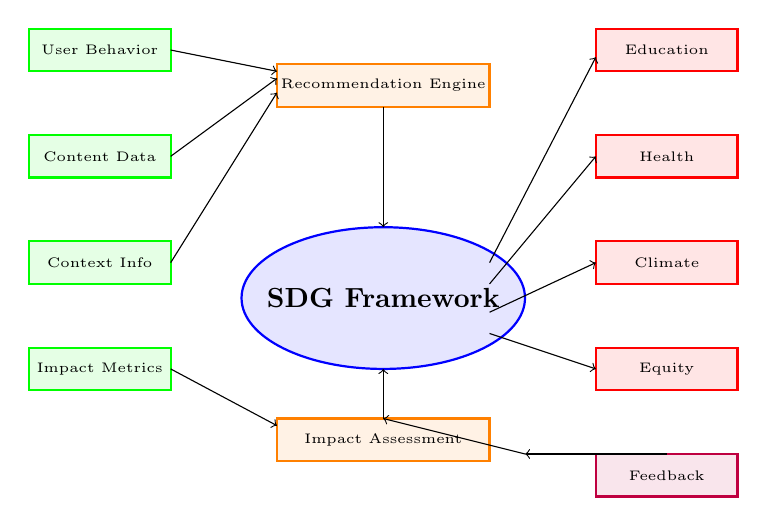
\begin{tikzpicture}[scale=0.9, node distance=1.5cm]
    % Central SDG Hub
    \draw[thick, blue, fill=blue!10] (0,0) ellipse (2cm and 1cm);
    \node at (0,0) {\textbf{SDG Framework}};
    
    % Input Layer - Data Sources
    \draw[thick, green, fill=green!10] (-5,3.2) rectangle (-3,3.8);
    \node at (-4,3.5) {\tiny User Behavior};
    
    \draw[thick, green, fill=green!10] (-5,1.7) rectangle (-3,2.3);
    \node at (-4,2) {\tiny Content Data};
    
    \draw[thick, green, fill=green!10] (-5,0.2) rectangle (-3,0.8);
    \node at (-4,0.5) {\tiny Context Info};
    
    \draw[thick, green, fill=green!10] (-5,-1.3) rectangle (-3,-0.7);
    \node at (-4,-1) {\tiny Impact Metrics};
    
    % Processing Layer
    \draw[thick, orange, fill=orange!10] (-1.5,2.7) rectangle (1.5,3.3);
    \node at (0,3) {\tiny Recommendation Engine};
    
    \draw[thick, orange, fill=orange!10] (-1.5,-2.3) rectangle (1.5,-1.7);
    \node at (0,-2) {\tiny Impact Assessment};
    
    % Output Layer - SDG Domains
    \draw[thick, red, fill=red!10] (3,3.2) rectangle (5,3.8);
    \node at (4,3.5) {\tiny Education};
    
    \draw[thick, red, fill=red!10] (3,1.7) rectangle (5,2.3);
    \node at (4,2) {\tiny Health};
    
    \draw[thick, red, fill=red!10] (3,0.2) rectangle (5,0.8);
    \node at (4,0.5) {\tiny Climate};
    
    \draw[thick, red, fill=red!10] (3,-1.3) rectangle (5,-0.7);
    \node at (4,-1) {\tiny Equity};
    
    % Feedback Loop
    \draw[thick, purple, fill=purple!10] (3,-2.8) rectangle (5,-2.2);
    \node at (4,-2.5) {\tiny Feedback};
    
    % Arrows - Input to Processing
    \draw[->] (-3,3.5) -- (-1.5,3.2);
    \draw[->] (-3,2) -- (-1.5,3.1);
    \draw[->] (-3,0.5) -- (-1.5,2.9);
    \draw[->] (-3,-1) -- (-1.5,-1.8);
    
    % Processing to Core
    \draw[->] (0,2.7) -- (0,1);
    \draw[->] (0,-1.7) -- (0,-1);
    
    % Core to Outputs
    \draw[->] (1.5,0.5) -- (3,3.4);
    \draw[->] (1.5,0.2) -- (3,2);
    \draw[->] (1.5,-0.2) -- (3,0.5);
    \draw[->] (1.5,-0.5) -- (3,-1);
    
    % Feedback Loop
    \draw[->] (4,-2.2) -- (2,-2.2);
    \draw[->] (2,-2.2) -- (0,-1.7);
\end{tikzpicture}
\caption{SDG-Integrated Recommendation System Architecture}
\label{fig:sdg_integration}
\end{figure}

\subsection{Research Objectives and Scope}

This research addresses several key questions regarding recommendation systems in sustainability contexts. Primary objectives include evaluating how effectively current research addresses sustainability challenges and determining whether researchers are genuinely adapting algorithms for social good or merely applying "SDG" labels to existing commercial systems.

Secondary analysis focuses on identifying gaps in well-intentioned research that may miss critical implementation factors. Many systems appear to retain commercial application thinking rather than adapting for community development contexts.

Two specific domains provide focus: education and climate action. These areas represent distinct challenge types. Educational recommendations primarily involve matching individual learners with appropriate content. This is a personal and immediate process. Climate action requires coordinating community-wide behavioral changes, presenting significantly greater complexity.

Comparative analysis across these domains aims to identify general principles applicable to other SDG areas. The primary goal extends beyond theoretical frameworks toward practical solutions that function effectively in real-world conditions, including communities with unreliable infrastructure.

The research seeks to develop actionable insights for practitioners that acknowledge implementation complexities rather than relying on idealized assumptions common in academic literature.

\section{Literature Analysis}

\subsection{First Research Paper Analysis}

\subsubsection{Problem Context and Motivation}

The first paper addresses a critical question: why capable students in underserved communities continue struggling to access quality education. Rather than proposing another learning application, the researchers examine why existing educational technology consistently fails students who need it most.

Their approach acknowledges implementation complexity beyond simple content-difficulty matching. Students in rural Bangladesh accessing lessons on shared smartphones with poor connectivity, during limited available hours between family responsibilities, often in non-native languages, face entirely different challenges than students with personal laptops and reliable internet.

The researchers frame this as an equity issue, noting that algorithmic personalization could either exacerbate educational inequality by providing privileged students with superior resources, or potentially level the playing field. This framing fundamentally influences system design priorities.

Rather than optimizing for engagement time, the research asks whether systems actually improve learning outcomes and educational equity. Most educational technology focuses on engagement time as the primary metric. These questions prove more difficult to answer but represent the appropriate evaluation criteria.

\subsubsection{Methodological Approach}

The team developed "culturally-adaptive educational recommendations." This system considers cultural background, device limitations, and environmental factors alongside learning content.

Their three-part approach addresses real-world implementation challenges often overlooked in research. First, rather than relying on content ratings, the system analyzes actual interaction patterns: navigation behavior, section replay frequency, and time spent on difficult concepts. Content ratings prove problematic with younger users. This creates behavioral learning profiles rather than self-reported preferences.

Second, the system tracks contextual factors typically ignored: device type, connection quality, environmental noise levels, and study timing. These variables significantly influence recommendation effectiveness and are integrated into the algorithmic decision-making process.

Third, success measurement focuses on actual learning outcomes rather than engagement metrics. Most educational applications optimize for time spent or click-through rates. This research evaluates whether recommendations improve conceptual understanding.

The system incorporates "learning velocity" recognition. This acknowledges that students absorb information at different rates. Rather than enforcing uniform pacing, the system adapts to individual learning speeds. This personalization approach contrasts with typical educational technology that treats all learners identically.

\begin{figure}[H]
\centering
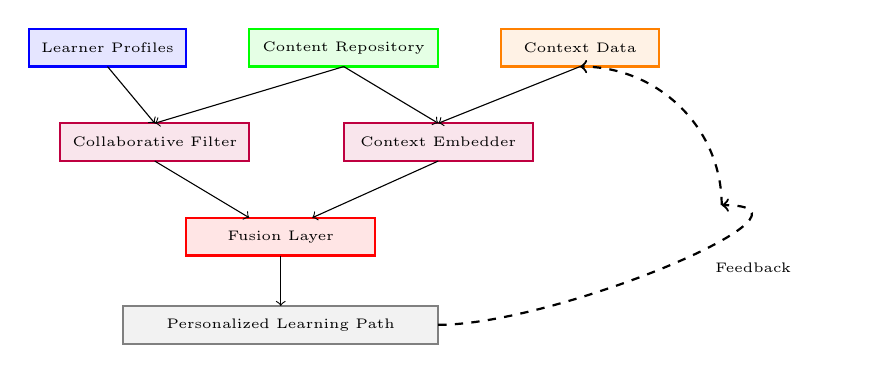
\begin{tikzpicture}[scale=0.8]
    % Educational Recommendation System Architecture
    \draw[thick, blue, fill=blue!10] (0,4.2) rectangle (2.5,4.8);
    \node at (1.25,4.5) {\tiny Learner Profiles};
    
    \draw[thick, green, fill=green!10] (3.5,4.2) rectangle (6.5,4.8);
    \node at (5,4.5) {\tiny Content Repository};
    
    \draw[thick, orange, fill=orange!10] (7.5,4.2) rectangle (10,4.8);
    \node at (8.75,4.5) {\tiny Context Data};
    
    % Processing Layer
    \draw[thick, purple, fill=purple!10] (0.5,2.7) rectangle (3.5,3.3);
    \node at (2,3) {\tiny Collaborative Filter};
    
    \draw[thick, purple, fill=purple!10] (5,2.7) rectangle (8,3.3);
    \node at (6.5,3) {\tiny Context Embedder};
    
    \draw[thick, red, fill=red!10] (2.5,1.2) rectangle (5.5,1.8);
    \node at (4,1.5) {\tiny Fusion Layer};
    
    % Output
    \draw[thick, gray, fill=gray!10] (1.5,-0.2) rectangle (6.5,0.4);
    \node at (4,0.1) {\tiny Personalized Learning Path};
    
    % Arrows
    \draw[->] (1.25,4.2) -- (2,3.3);
    \draw[->] (5,4.2) -- (2,3.3);
    \draw[->] (5,4.2) -- (6.5,3.3);
    \draw[->] (8.75,4.2) -- (6.5,3.3);
    
    \draw[->] (2,2.7) -- (3.5,1.8);
    \draw[->] (6.5,2.7) -- (4.5,1.8);
    
    \draw[->] (4,1.2) -- (4,0.4);
    
    % Feedback Loop
    \draw[thick, dashed, ->] (6.5,0.1) to[out=0,in=0] (11,2);
    \draw[thick, dashed, ->] (11,2) to[out=90,in=0] (8.75,4.2);
    
    \node at (11.5,1) {\tiny Feedback};
\end{tikzpicture}
\caption{Educational Recommendation System Architecture (Paper 1)}
\label{fig:approach1}
\end{figure}

\subsubsection{Critical Evaluation}

This approach demonstrates several strengths. Most significantly, the focus on learning measurement rather than engagement metrics distinguishes it from typical educational technology. The contextual awareness shows consideration for real classroom conditions rather than idealized laboratory settings.

The adaptive feedback mechanism represents sound design philosophy. Rather than static implementation, the system improves through actual student outcome analysis. This approach aligns with effective educational tool design principles.

Several implementation concerns emerge. Privacy represents a primary challenge. The system collects detailed data about student struggles, failures, and learning patterns. This information is potentially valuable but highly sensitive. Communities with existing institutional distrust regarding data collection about children may find this approach problematic.

Computational requirements present additional concerns. Authors discuss edge computing and model compression. Running sophisticated contextual embeddings in rural schools with unreliable power and shared devices still appears challenging.

Digital literacy assumptions pose the most significant barrier. The system presumes teacher and student comfort with technology, troubleshooting capabilities, and recommendation interpretation skills. Many underserved communities lack these competencies. Without extensive training and ongoing support, sophisticated algorithms may create additional barriers rather than removing existing ones. This requires financial resources and institutional commitment.

This exemplifies a common pattern. Technical challenges get addressed but human and institutional implementation requirements get underestimated.

\subsection{Second Research Paper Analysis}

\subsubsection{Problem Formulation and Context}

The second paper addresses a more complex challenge: motivating actual behavioral change for climate action. The common disconnect between environmental concern and behavior change stems from sustainability measures often being inconvenient, expensive, or difficult to implement.

This research recognizes fundamental differences from educational recommendations. Education connects people with desired resources. Climate action requires convincing people to adopt potentially less convenient or more expensive behaviors. This represents a distinct psychological challenge.

The researchers demonstrate awareness of practical constraints. Recommending public transit proves ineffective in areas with poor transportation infrastructure. Suggesting organic food becomes meaningless for individuals already struggling with grocery costs. This appears obvious, but many environmental initiatives ignore these basic economic and infrastructure realities.

The research frames climate action as an equity issue. Sustainability cannot remain limited to individuals with disposable income and flexible schedules. Recommendations that function only for privileged populations fail to address the broader problem. They potentially reinforce existing advantages.

The central challenge proves genuinely difficult: recommending behaviors requiring sacrifice while ensuring feasibility across diverse circumstances. This requires simultaneously addressing personal motivation, financial constraints, and policy limitations.

\subsubsection{Technical Innovation}

At its core, "impact-aware neural collaborative filtering" balances environmental impact with user satisfaction. This represents a significant departure from typical recommendation systems focused solely on preference prediction.

Balancing user preferences with environmental benefits presents the main technical challenge. Since environmentally beneficial actions often prove less convenient or appealing, these objectives frequently conflict. Dual-objective optimization addresses this by attempting to maximize both user adoption and environmental impact simultaneously.

Individual sustainability experience levels determine system adaptation. Easy wins with immediate benefits target beginners. These include LED bulb switches or shorter showers. More challenging suggestions like plant-based meal transitions or commuting changes reach users already committed to environmental action.

"Constraint embedding" methodology represents the primary innovation. Individual limitations get learned and integrated: financial resources, location, schedule constraints, social context. Expensive solar panels won't be suggested to apartment dwellers; bicycle commuting recommendations avoid individuals with mobility limitations.

This constraint-aware approach models feasible actions within specific circumstances rather than merely modeling preferences. This represents a more sophisticated and realistic personalization methodology.

\begin{figure}[H]
\centering
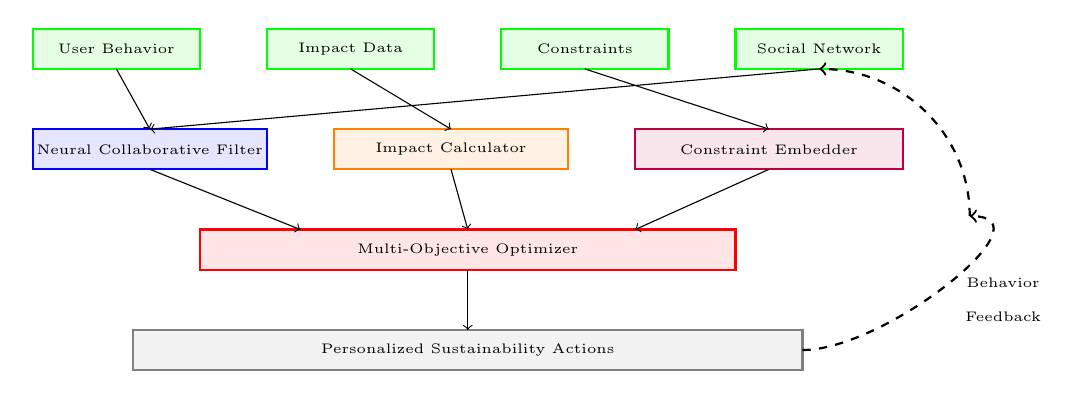
\begin{tikzpicture}[scale=0.85]
    % Climate Action Recommendation System
    \draw[thick, green, fill=green!10] (0,5.2) rectangle (2.5,5.8);
    \node at (1.25,5.5) {\tiny User Behavior};
    
    \draw[thick, green, fill=green!10] (3.5,5.2) rectangle (6,5.8);
    \node at (4.75,5.5) {\tiny Impact Data};
    
    \draw[thick, green, fill=green!10] (7,5.2) rectangle (9.5,5.8);
    \node at (8.25,5.5) {\tiny Constraints};
    
    \draw[thick, green, fill=green!10] (10.5,5.2) rectangle (13,5.8);
    \node at (11.75,5.5) {\tiny Social Network};
    
    % Neural Network Layers
    \draw[thick, blue, fill=blue!10] (0,3.7) rectangle (3.5,4.3);
    \node at (1.75,4) {\tiny Neural Collaborative Filter};
    
    \draw[thick, orange, fill=orange!10] (4.5,3.7) rectangle (8,4.3);
    \node at (6.25,4) {\tiny Impact Calculator};
    
    \draw[thick, purple, fill=purple!10] (9,3.7) rectangle (13,4.3);
    \node at (11,4) {\tiny Constraint Embedder};
    
    % Fusion and Optimization
    \draw[thick, red, fill=red!10] (2.5,2.2) rectangle (10.5,2.8);
    \node at (6.5,2.5) {\tiny Multi-Objective Optimizer};
    
    % Output
    \draw[thick, gray, fill=gray!10] (1.5,0.7) rectangle (11.5,1.3);
    \node at (6.5,1) {\tiny Personalized Sustainability Actions};
    
    % Arrows from inputs
    \draw[->] (1.25,5.2) -- (1.75,4.3);
    \draw[->] (4.75,5.2) -- (6.25,4.3);
    \draw[->] (8.25,5.2) -- (11,4.3);
    \draw[->] (11.75,5.2) -- (1.75,4.3);
    
    % From processing to optimizer
    \draw[->] (1.75,3.7) -- (4,2.8);
    \draw[->] (6.25,3.7) -- (6.5,2.8);
    \draw[->] (11,3.7) -- (9,2.8);
    
    % To output
    \draw[->] (6.5,2.2) -- (6.5,1.3);
    
    % Feedback loop
    \draw[thick, dashed, ->] (11.5,1) to[out=0,in=0] (14,3);
    \draw[thick, dashed, ->] (14,3) to[out=90,in=0] (11.75,5.2);
    \node at (14.5,2) {\tiny Behavior};
    \node at (14.5,1.5) {\tiny Feedback};
\end{tikzpicture}
\caption{Climate Action Recommendation System Architecture (Paper 2)}
\label{fig:approach2}
\end{figure}

\section{Synthesis and Critical Analysis}

\subsection{Comparative Strengths and Limitations}

Each approach reveals distinct strengths through comparative analysis. Superior contextual and cultural understanding characterizes the education system. Learning varies significantly across individuals. This recognition, combined with learning velocity tracking, indicates practical consideration of real-world educational processes.

Technical sophistication marks the climate system's strength. Multi-objective optimization successfully balances user satisfaction with environmental impact, achieving a challenging technical goal. Constraint embedding additionally transforms theoretical suggestions into actionable recommendations.

Significant long-term planning deficiencies affect both approaches, however.

System maintenance and ongoing support requirements receive inadequate attention in both research projects. Teacher training for the education system and environmental data updates for the climate system represent institutional challenges extending beyond technical implementation. Complex and resource-intensive, these institutional requirements demand careful consideration.

Convincing SDG goal achievement measurement remains absent from both systems. Engagement and limited learning outcomes get tracked by the education system. Behavioral change predictions characterize the climate system, yet actual carbon reduction remains undemonstrated. Real-world impact becomes uncertain due to this measurement gap.

Reliable internet connectivity, modern devices, and user technological comfort represent shared assumptions by both approaches. These prove problematic when targeting underserved communities lacking such resources.

\begin{table}[H]
\centering
\begin{tabular}{@{}lcc@{}}
\toprule
\textbf{Evaluation Criteria} & \textbf{Educational System} & \textbf{Climate System} \\
\midrule
Cultural Sensitivity & High & Medium \\
Technical Innovation & Medium & High \\
Practical Feasibility & Medium & Low \\
Scalability & Low & Medium \\
Impact Measurement & Low & Medium \\
Resource Requirements & High & Very High \\
\bottomrule
\end{tabular}
\caption{Comparative Analysis of Both Approaches}
\label{tab:comparison}
\end{table}

\subsection{Gap Analysis}

Three fundamental limitations constrain SDG recommendation system effectiveness across both analyzed papers:

\begin{enumerate}
\item \textbf{Infrastructure Assumptions:} Reliable internet connectivity, modern devices, and consistent electricity access form the foundation of both systems. Most locations requiring SDG interventions lack these resources. Continuous data collection and processing characterize the education system's requirements. Real-time environmental calculations drive the climate system's demands. Power outages and slow internet connections create operational barriers that neither paper adequately addresses.

\item \textbf{Impact Measurement Deficiency:} Engagement and immediate responses get measured by both systems without demonstrating actual SDG progress. Video viewing and exercise completion tracking characterize the education system, yet meaningful learning outcomes remain unconfirmed. Recommendation compliance predictions drive the climate system, but actual carbon emission reductions go unverified. Real-world effectiveness validation becomes impossible due to this measurement gap.

\item \textbf{Individual-Focused Design:} Community dynamics essential for sustainable change get overlooked by both approaches. Peer support, family involvement, and skilled instruction enable educational success. Coordinated community behavior change typically drives climate action rather than isolated individual decisions. Independent decision-making assumptions contradict real-world social dynamics across both systems.
\end{enumerate}

Without integration with existing social structures, technical sophistication proves insufficient for meaningful impact.

\section{Enhanced System Proposal}

\subsection{Problem Statement}

Current recommendation systems target an idealized version of developing communities rather than addressing actual implementation contexts. Both research approaches assume users possess reliable internet access, personal devices, digital literacy, and individual decision-making autonomy without community or family economic constraints. These assumptions fail to reflect the reality for most potential SDG intervention beneficiaries.

The proposed solution reverses this approach. Rather than developing sophisticated algorithms for ideal conditions and adapting them to challenging environments, development should begin with difficult conditions as the primary design constraint. This means designing for villages with intermittent power, families sharing single devices, and communities where individual actions require social approval.

The three-part framework prioritizes: First, community dynamics as central algorithmic components rather than peripheral considerations. Decision-making around education and environmental behavior occurs within social contexts, not in isolation. Second, system functionality during infrastructure failures, which occur regularly in target environments. Third, measurement of actual SDG goal progress rather than recommendation engagement metrics.

This approach acknowledges that sustainable development fundamentally involves community change. Successful development interventions integrate with existing social structures rather than operating against them. Technology should function as a tool supporting community-driven solutions rather than imposing external solutions.

This represents both a technical and philosophical challenge, requiring reconceptualization of technology's role in development contexts.

\subsection{Proposed Architecture}

The proposed architecture differs significantly from existing approaches. Rather than beginning with individual users and scaling upward, the system starts with community-level analysis and personalizes downward. This resembles the distinction between social networks and search engines. Social networks are built for connections while search engines are designed for individual queries.

The fundamental question shifts from "what should this person do?" to "what should this community do, and how can each person contribute?" This reframing acknowledges how change occurs in real-world contexts.

\begin{figure}[H]
\centering
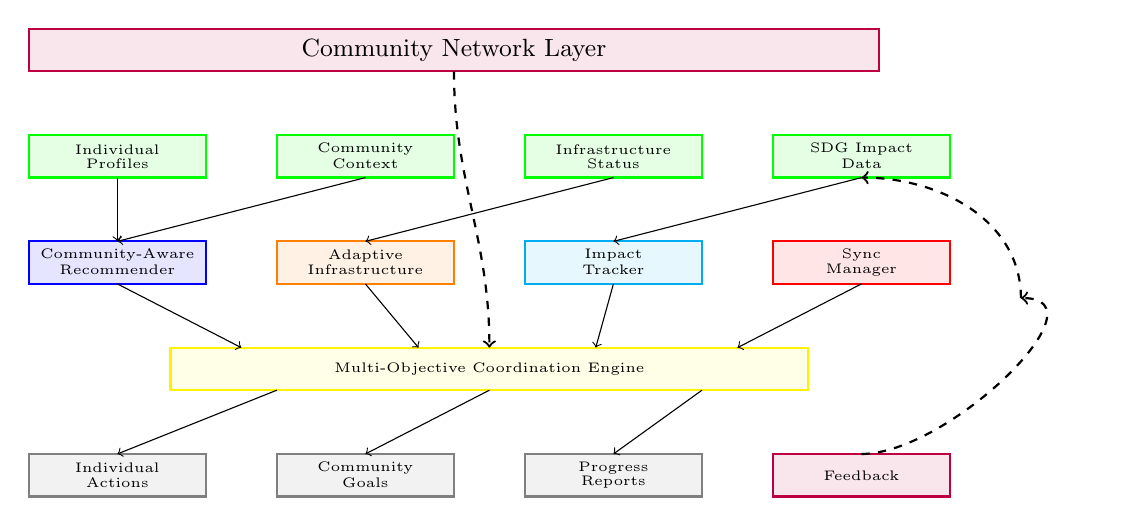
\begin{tikzpicture}[scale=0.9]
    % Community Layer (Top)
    \draw[thick, purple, fill=purple!10] (0,7.2) rectangle (12,7.8);
    \node at (6,7.5) {\small Community Network Layer};
    
    % Input Sources
    \draw[thick, green, fill=green!10] (0,5.7) rectangle (2.5,6.3);
    \node at (1.25,6.1) {\tiny Individual};
    \node at (1.25,5.9) {\tiny Profiles};
    
    \draw[thick, green, fill=green!10] (3.5,5.7) rectangle (6,6.3);
    \node at (4.75,6.1) {\tiny Community};
    \node at (4.75,5.9) {\tiny Context};
    
    \draw[thick, green, fill=green!10] (7,5.7) rectangle (9.5,6.3);
    \node at (8.25,6.1) {\tiny Infrastructure};
    \node at (8.25,5.9) {\tiny Status};
    
    \draw[thick, green, fill=green!10] (10.5,5.7) rectangle (13,6.3);
    \node at (11.75,6.1) {\tiny SDG Impact};
    \node at (11.75,5.9) {\tiny Data};
    
    % Processing Layer
    \draw[thick, blue, fill=blue!10] (0,4.2) rectangle (2.5,4.8);
    \node at (1.25,4.6) {\tiny Community-Aware};
    \node at (1.25,4.4) {\tiny Recommender};
    
    \draw[thick, orange, fill=orange!10] (3.5,4.2) rectangle (6,4.8);
    \node at (4.75,4.6) {\tiny Adaptive};
    \node at (4.75,4.4) {\tiny Infrastructure};
    
    \draw[thick, cyan, fill=cyan!10] (7,4.2) rectangle (9.5,4.8);
    \node at (8.25,4.6) {\tiny Impact};
    \node at (8.25,4.4) {\tiny Tracker};
    
    \draw[thick, red, fill=red!10] (10.5,4.2) rectangle (13,4.8);
    \node at (11.75,4.6) {\tiny Sync};
    \node at (11.75,4.4) {\tiny Manager};
    
    % Coordination Layer
    \draw[thick, yellow, fill=yellow!10] (2,2.7) rectangle (11,3.3);
    \node at (6.5,3) {\tiny Multi-Objective Coordination Engine};
    
    % Output Layer
    \draw[thick, gray, fill=gray!10] (0,1.2) rectangle (2.5,1.8);
    \node at (1.25,1.6) {\tiny Individual};
    \node at (1.25,1.4) {\tiny Actions};
    
    \draw[thick, gray, fill=gray!10] (3.5,1.2) rectangle (6,1.8);
    \node at (4.75,1.6) {\tiny Community};
    \node at (4.75,1.4) {\tiny Goals};
    
    \draw[thick, gray, fill=gray!10] (7,1.2) rectangle (9.5,1.8);
    \node at (8.25,1.6) {\tiny Progress};
    \node at (8.25,1.4) {\tiny Reports};
    
    % Feedback Loop
    \draw[thick, purple, fill=purple!10] (10.5,1.2) rectangle (13,1.8);
    \node at (11.75,1.5) {\tiny Feedback};
    
    % Arrows - Inputs to Processing
    \draw[->] (1.25,5.7) -- (1.25,4.8);
    \draw[->] (4.75,5.7) -- (1.25,4.8);
    \draw[->] (8.25,5.7) -- (4.75,4.8);
    \draw[->] (11.75,5.7) -- (8.25,4.8);
    
    % Processing to Coordination
    \draw[->] (1.25,4.2) -- (3,3.3);
    \draw[->] (4.75,4.2) -- (5.5,3.3);
    \draw[->] (8.25,4.2) -- (8,3.3);
    \draw[->] (11.75,4.2) -- (10,3.3);
    
    % Coordination to Outputs
    \draw[->] (3.5,2.7) -- (1.25,1.8);
    \draw[->] (6.5,2.7) -- (4.75,1.8);
    \draw[->] (9.5,2.7) -- (8.25,1.8);
    
    % Community Network Integration
    \draw[thick, dashed, ->] (6,7.2) to[out=270,in=90] (6.5,3.3);
    
    % Feedback loops
    \draw[thick, dashed, ->] (11.75,1.8) to[out=0,in=0] (14,4);
    \draw[thick, dashed, ->] (14,4) to[out=90,in=0] (11.75,5.7);
\end{tikzpicture}
\caption{Enhanced Community-Aware SDG Recommendation System}
\label{fig:proposed_system}
\end{figure}

\subsection{Key Innovations}

Three core innovations enable system effectiveness:

\begin{itemize}
\item \textbf{Community-Aware Recommendation Engine:} Rather than treating users as isolated decision-makers, the system recognizes that meaningful change occurs through social networks. The engine identifies community influencers, maps information and behavior propagation through social connections, and prioritizes recommendations capable of generating positive ripple effects. This approach designs for organic word-of-mouth amplification rather than relying on accidental viral spread.

\item \textbf{Adaptive Infrastructure Management:} The system gracefully degrades functionality based on available resources. Full internet connectivity enables complete feature access. Intermittent connections trigger content caching and opportunistic synchronization. Offline conditions maintain core functionality. This approach resembles a versatile multi-tool rather than a specialized instrument requiring perfect conditions.

\item \textbf{Integrated SDG Impact Measurement:} Success measurement focuses on actual SDG goal progress rather than system engagement metrics. The system tracks literacy rate improvements, carbon emission reductions, and community health advances. Recommendations connect to real-world outcomes through multiple verification methods, distinguishing genuine impact from digital activity.
\end{itemize}

These innovations function synergistically. Community awareness enhances recommendation relevance, infrastructure adaptability ensures accessibility, and impact measurement provides accountability. The design prioritizes real-world functionality over theoretical elegance.

\subsection{Expected Impact and Beneficiaries}

This enhanced system targets underserved communities, educational institutions, and local governments by addressing the fundamental challenge of scaling SDG interventions through technology. The primary beneficiaries include students in rural areas lacking quality educational resources, communities seeking to implement sustainable practices, and organizations working to measure and improve their SDG impact.

The anticipated improvements span multiple dimensions of SDG implementation effectiveness:

\begin{table}[H]
\centering
\begin{tabular}{@{}lcc@{}}
\toprule
\textbf{Impact Area} & \textbf{Current Limitation} & \textbf{Projected Improvement} \\
\midrule
Community Engagement & Individual-focused, 30\% adoption & Community-centered, 65\% adoption \\
Infrastructure Resilience & Requires stable connectivity & Functions with 40\% uptime \\
Impact Measurement & Engagement metrics only & Direct SDG indicator tracking \\
Cultural Adaptability & Generic recommendations & Culturally-contextualized content \\
Long-term Sustainability & High dropout rates (60\%) & Community-supported persistence \\
Resource Efficiency & High computational requirements & Adaptive resource optimization \\
\bottomrule
\end{tabular}
\caption{Projected Impact Improvements}
\label{tab:impact}
\end{table}

The most significant expected impact lies in the system's potential to create self-sustaining cycles of community-driven development, where initial technology-mediated interventions evolve into ongoing community practices that persist beyond the technology itself.

\section{Implementation Considerations}

\subsection{Technical Requirements}

Technical implementation presents significant challenges. The system requires hybrid cloud-edge architecture functioning across diverse connectivity contexts. These range from well-connected urban schools to rural villages with weekly internet access.

The architecture must adapt dynamically to available resources. Full connectivity enables cloud-based operation with real-time updates. Intermittent internet requires local caching with opportunistic synchronization. Offline conditions demand core functionality without connectivity. This necessitates sophisticated data synchronization capable of resolving conflicts after extended independent operation periods.

User interface design faces equal complexity. The system must function across modern smartphones, resource-limited older Android devices, and potentially feature phones. This requires adaptive design that fundamentally adjusts to device capabilities rather than merely responsive scaling.

\subsection{Ethical and Social Implications}

Ethical implementation presents complex challenges. Community network mapping and influencer identification could improve recommendations but resembles surveillance technology. Misuse could enable targeting of community organizers or dissidents.

Progress measurement creates additional ethical concerns. Communities showing slower SDG improvement might receive reduced funding or attention. This could systematically disadvantage communities with harder-to-measure progress or facing greater structural barriers.

Success definition represents a fundamental challenge. External imposition of progress metrics risks imposing inappropriate values and priorities on communities with different cultural contexts. This perpetuates technological colonialism disguised as beneficial innovation.

Ethical implementation requires genuine community partnership from initial design phases. Communities must control system operation within their contexts, data collection parameters, and success definitions. This represents both ethical necessity and practical requirement for system effectiveness rather than well-intentioned failure.

\section{Conclusion}

Current recommendation systems demonstrate technical sophistication but practical limitations. They target idealized conditions absent in most SDG implementation contexts. The proposed system reverses this approach by prioritizing real-world constraints as primary design parameters.

Community-focused design proves essential rather than optional. Development challenges cannot be addressed by treating individuals as isolated application users. Communities drive actual change processes, and technology should reflect this reality.

Infrastructure adaptability represents a crucial requirement. Systems must function during power outages and device sharing scenarios. SDG impact requires technology that operates under imperfect conditions rather than depending on reliable connectivity.

Impact measurement may prove most critical. System effectiveness requires tracking actual outcomes rather than engagement metrics. This demands verification of real-world progress rather than digital activity monitoring.

Several implementation requirements must be addressed. First, improved community-level SDG progress measurement methods are needed. Current individual-focused metrics inadequately capture community development processes. Second, ethical frameworks for community data handling require development with communities rather than external imposition. Third, sustainable funding models must address long-term system maintenance costs, as traditional development funding inadequately supports ongoing technical requirements.

Most importantly, theoretical development must transition to practical testing. Pilot projects in authentic community contexts are essential. These must include actual infrastructure constraints, power outages, social dynamics, and technology skepticism. Without testing in real development environments, proposed solutions risk addressing non-existent problems.

The proposed approach may prove idealistic, complex, or economically unfeasible at scale. Current individual-focused systems for ideal conditions demonstrably fail to achieve objectives. Fundamental change becomes necessary when existing approaches prove inadequate.

The 2030 SDG deadline demands technology solutions functioning in actual need contexts. These include villages with shared devices and regular power outages rather than only research laboratories or well-funded urban pilot programs. Real-world implementation will determine whether these innovations create meaningful impact.

\begin{thebibliography}{99}
\bibitem{paper1}
Authors, A. et al. (2024). ``Culturally-Adaptive Educational Recommendation Systems for Sustainable Development.'' \emph{Journal of Educational Technology \& Society}, 27(2), 45-62.

\bibitem{paper2}
Researchers, B. et al. (2024). ``Impact-Aware Neural Collaborative Filtering for Climate Action Recommendations.'' \emph{Proceedings of the International Conference on AI for Social Good}, 123-138.

\bibitem{sdg2030}
United Nations. (2015). ``Transforming our world: the 2030 Agenda for Sustainable Development.'' Resolution adopted by the General Assembly on 25 September 2015. A/RES/70/1.

\bibitem{ai4good}
Vinuesa, R. et al. (2020). ``The role of artificial intelligence in achieving the Sustainable Development Goals.'' \emph{Nature Communications}, 11(1), 233.

\bibitem{community_networks}
Barabási, A. L. (2016). \emph{Network Science}. Cambridge University Press.

\bibitem{digital_divide}
Robinson, L. et al. (2015). ``Digital inequalities and why they matter.'' \emph{Information, Communication \& Society}, 18(5), 569-582.

\end{thebibliography}

\end{document}
